% Dit werk is gelicenseerd onder de licentie Creative Commons Naamsvermelding-GelijkDelen 4.0 Internationaal. Ga naar http://creativecommons.org/licenses/by-sa/4.0/ om een kopie van de licentie te kunnen lezen.
\chapter{Behoudsvergelijkingen}
\label{sec:Behoudsvergelijkingen}
%%%%%%%%%%%%%%%%%%%%%%%%%%%%%%%%%%%%%%%%%%%%%%%%%%%%%%%%%%%%%%%%%%%%%%%%%%%%%%%%%%%%%%%%%
\begin{toepassing}[*]
	\label{waterkraan}
Uit een kraan stroomt water verticaal naar beneden met een debiet van 5 l/min. Tegen de kraan heeft de waterstraal een diameter van 18 mm. 

Bepaal de diameter van de waterstraal op een afstand van 0.2 m onder de kraan.

	\centering
	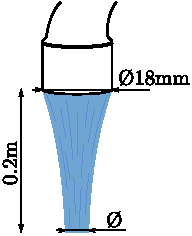
\includegraphics{fig/behoudsvergelijkingen/waterkraan}

\end{toepassing}
\begin{antwoord}{\ref{waterkraan}}
	$d = 7.3 \unit{mm}$
\end{antwoord}
%%%%%%%%%%%%%%%%%%%%%%%%%%%%%%%%%%%%%%%%%%%%%%%%%%%%%%%%%%%%%%%%%%%%%%%%%%%%%%%%%%%%%%%%%
\begin{toepassing}[*]
	\label{hevel}
Een hevel wordt gebruikt om water uit een tank te halen, aan het uiteinde van de hevel heerst de atmosfeerdruk. De hoogtes zijn zoals aangegeven op onderstaande figuur, de buis heeft een constante diameter. Veronderstel dat het water zich niet viskeus gedraagt.
		
Bepaal de gemiddelde snelheid en de druk op het hoogste punt in de hevel.

	\centering
	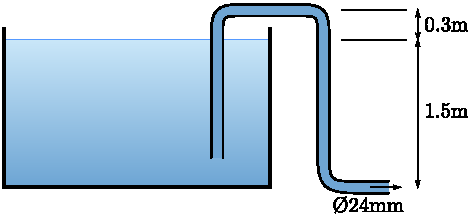
\includegraphics{fig/behoudsvergelijkingen/hevel}

\end{toepassing}
\begin{antwoord}{\ref{hevel}}
	$v = 5.42 \unit{m/s}$, $p = 84 \unit{kPa}$
\end{antwoord}
%%%%%%%%%%%%%%%%%%%%%%%%%%%%%%%%%%%%%%%%%%%%%%%%%%%%%%%%%%%%%%%%%%%%%%%%%%%%%%%%%%%%%%%%%
\begin{toepassing}
	\label{drukhoogte}
Een leidingstelsel is opgebouwd zoals weergegeven in onderstaande figuur. Er zijn twee verticale meetbuizen aangebracht om de druk in de leidingen te kunnen meten. In de leidingen stroomt water dat als niet viskeus beschouwd mag worden.
		
Bepaal de hoogte van de vloeistof in de twee meetbuizen t.o.v. het vloeistof niveau in de tank.

	\centering
	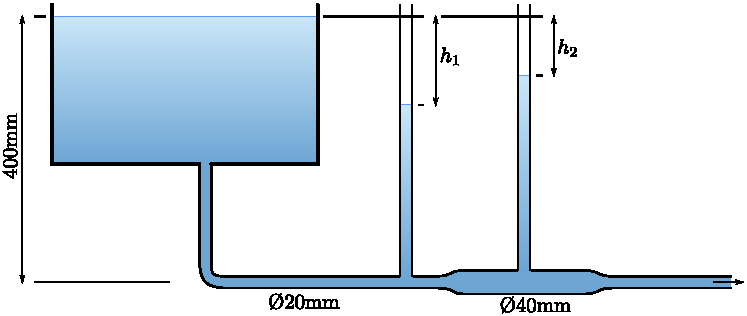
\includegraphics{fig/behoudsvergelijkingen/drukhoogte}
\end{toepassing}
\begin{antwoord}{\ref{drukhoogte}}
	$h_1 = 400 \unit{mm}$, $h_2 = 25 \unit{mm}$
\end{antwoord}
%%%%%%%%%%%%%%%%%%%%%%%%%%%%%%%%%%%%%%%%%%%%%%%%%%%%%%%%%%%%%%%%%%%%%%%%%%%%%%%%%%%%%%%%%
\begin{toepassing}
	\label{dynamische_druk}
Een een Pitot-buis en een manometer aangesloten op een leiding waarin lucht stroomt ($\rho=1.22 \unit{kg/m^3}$). Beide buizen zijn aangesloten op een U-buis manometer waarin een olie met een dichtheid van $800 \unit{kg/m^3}$ zit. De hoogteverschillen in de U-buizen zijn 0.2 m en 0.6 m zoals aangegeven op de figuur.

Bepaal de statische en de dynamische druk in de buis en de snelheid in de buis.

	\centering
	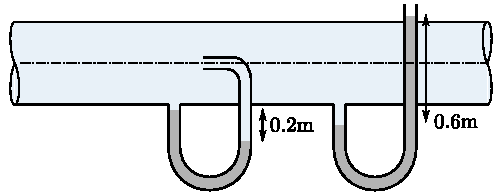
\includegraphics{fig/behoudsvergelijkingen/dynamische_druk}
\end{toepassing}
\begin{antwoord}{\ref{dynamische_druk}}
	$p_{\text{statisch}} = 4709 \unit{Pa}$, $p_{\text{dynamisch}} = 1570 \unit{Pa}$,\\ $v = 50.7 \unit{m/s}$
\end{antwoord}
%%%%%%%%%%%%%%%%%%%%%%%%%%%%%%%%%%%%%%%%%%%%%%%%%%%%%%%%%%%%%%%%%%%%%%%%%%%%%%%%%%%%%%%%%
\begin{toepassing}
	\label{annulair_controlevolume}
Door een annulair controle volume met gemiddelde straal 20 m, en dikte 1m stoomt lucht ($\rho=1.22 \unit{kg/m^3}$). Een voorwerp in het controlevolume beïnvloedt de stroming. Aan de ene zijde heeft de snelheid een axiale component van 10 m/s en een rotatiesnelheid van 1.26 rad/s. Aan de andere zijde is de rotatiesnelheid verhoogd tot 1.29 rad/s. Door de cilindrische zijwanden van het controlevolume is geen stroming.

Bepaal de axiale kracht uitgeoefend op het voorwerp in het controlevolume.
\end{toepassing}
\begin{antwoord}{\ref{annulair_controlevolume}}
	$F = 2.35 \unit{kN}$
\end{antwoord}
%%%%%%%%%%%%%%%%%%%%%%%%%%%%%%%%%%%%%%%%%%%%%%%%%%%%%%%%%%%%%%%%%%%%%%%%%%%%%%%%%%%%%%%%%
\begin{toepassing}
	\label{vernauwing}
Een vernauwing in een buis heeft afmetingen zoals afgebeeld op de onderstaande figuur. Door de buis stroomt olie met een dichtheid van $830 \unit{kg/m^3}$. De druk vlak voor de vernauwing is $2 \unit{bar}$. De stroming mag stationair en zonder wrijving verondersteld worden.
		
Bepaal de kracht uitgeoefend op de vernauwing ten gevolge van de stroming.

	\centering
	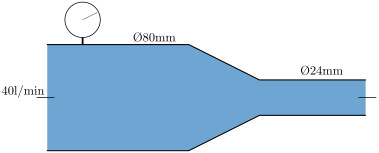
\includegraphics{fig/behoudsvergelijkingen/vernauwing}
\end{toepassing}
\begin{antwoord}{\ref{vernauwing}}
	$F = 919 \unit{N}$
\end{antwoord}
%%%%%%%%%%%%%%%%%%%%%%%%%%%%%%%%%%%%%%%%%%%%%%%%%%%%%%%%%%%%%%%%%%%%%%%%%%%%%%%%%%%%%%%%%
\begin{toepassing}
	\label{hydraulische_sprong}
In een hydraulisce sprong gaat een open kanaal stroming van hoge snelheid en een lage diepte naar een veel lagere snelheid en een grote diepte zoals aangegeven in onderstaande figuur. Dit gaat gepaard met grote energieverliezen. Indien de oorspronkelijke stroming ($\rho=1000 \unit{kg/m^3}$) een diepte van 0.20 m en een snelheid van 5 m/s heeft en de stoming als uniform beschouwd wordt en er geen weerstandskrachten optreden aan de bodem, bepaal dan de uiteindelijke diepte.

	\centering
	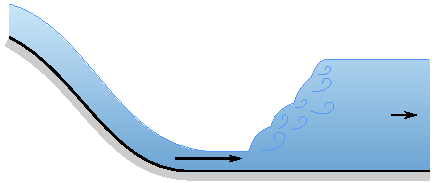
\includegraphics{fig/behoudsvergelijkingen/hydraulische_sprong}
\end{toepassing}
\begin{antwoord}{\ref{hydraulische_sprong}}
	$h = 0.91 \unit{m}$
\end{antwoord}
%%%%%%%%%%%%%%%%%%%%%%%%%%%%%%%%%%%%%%%%%%%%%%%%%%%%%%%%%%%%%%%%%%%%%%%%%%%%%%%%%%%%%%%%%
\begin{toepassing}[*]
	\label{brandslang}
Het uitlaatstuk van een brandslang vormt een vernauwing van de slang diameter (50 mm) tot de uitlaat (16 mm). De stroming hierin mag zonder wrijving verondersteld worden.

Bepaal de kracht die uitgeoefend wordt op het uitlaatstuk indien er een debiet van 180 l/min water door de slang stroomt en we de zwaartekracht niet beschouwen.

	\centering
	%\includegraphics{fig/behoudsvergelijkingen/brandslang}
\end{toepassing}
\begin{antwoord}{\ref{brandslang}}
	$F_x = 176 \unit{N}$
\end{antwoord}
%%%%%%%%%%%%%%%%%%%%%%%%%%%%%%%%%%%%%%%%%%%%%%%%%%%%%%%%%%%%%%%%%%%%%%%%%%%%%%%%%%%%%%%%%
\begin{toepassing}[*]
	\label{diffusiebocht}
Door een U-buis in een horizontaal vlak, met verlopende doorsnede, stroomt water met een intredesnelheid van 4 m/s. De oppervlaktes van de doorsneden bij in en uittrede zijn gegeven in de figuur. De druk aan de intrede wordt gemeten en is $150 \unit{kPa}$. De stroming mag als niet viskeus beschouwd worden.
		
Bepaal de grootte en de richting van de reactiekracht van de buis op het water.

	\centering
	
\includegraphics{fig/behoudsvergelijkingen/diffusiebocht}
\end{toepassing}
\begin{antwoord}{\ref{diffusiebocht}}
	$F = 97.2 \unit{kN}$
\end{antwoord}
%%%%%%%%%%%%%%%%%%%%%%%%%%%%%%%%%%%%%%%%%%%%%%%%%%%%%%%%%%%%%%%%%%%%%%%%%%%%%%%%%%%%%%%%%
\begin{toepassing}[*]
	\label{stofzuiger}
Een stofzuiger met een borstel accesoire zuigt een lucht debiet aan van $0.03 \unit{m^3/s}$ ($\rho=1.22 \unit{kg/m^3}$). De zuigmond maakt een hoek van 45\deg zoals aangegeven op de figuur. Indien de lucht uniform en volledig radiaal aangezogen wordt en de stroming verliesvrij verondersteld wordt, bepaal dan de kracht die op de zuigmond wordt uitgeoefend. Verwaarloos hoogteverschillen.

	\centering
	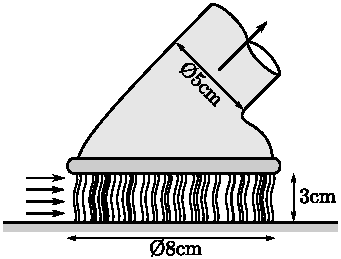
\includegraphics{fig/behoudsvergelijkingen/stofzuiger}
\end{toepassing}
\begin{antwoord}{\ref{stofzuiger}}
	$F_x = F_y = -0.21 \unit{N}$
\end{antwoord}	
%%%%%%%%%%%%%%%%%%%%%%%%%%%%%%%%%%%%%%%%%%%%%%%%%%%%%%%%%%%%%%%%%%%%%%%%%%%%%%%%%%%%%%%%%
\section*{Antwoorden}
	\begin{multicols}{2}
		\includecollection{antwoorden}
	\end{multicols}